% 附录 AL：非线性等离子体物理（从孤子到参量不稳定性与波崩塌）
% 数值唯一来源：tools/calc/appAL_calc.py -> tools/calc/appAL_calc.txt（本附录凡标出数字的量都由它复算）
% 工作点与附录 M/S/U/V/W/X/Y/Z/AD/AE/AI/AJ/AK 同一台：
%   n_e = 1e20 m^-3, T_e = 9.194 keV, B = 5.3 T, m_i = 2.5 m_p；
%   微波侧：140 GHz / 1 MW / 光斑 2 cm；激光侧：0.35 μm、冕区 n_e = 1e26 m^-3、T_e = 1 keV
% 单位写法：数字与单位都写进数学模式；中文只能放在 \text{} 里，不得进 \mathrm{}
% 约定：非线性判据一律写成无量纲比值（v_osc/v_the、U_p/T_e、a0）
% 版权口径：只借鉴结论、公式形式与题型，文字、数值与表格自拟并独立复算；
%   离线环境无法核验 DOI，故只给作者、书名/刊名、年份与卷期页
% 分工：附录 M 讲加热与电流驱动、附录 AE 讲动理学与Landau 阻尼、附录 AF 讲湍流谱、
%   附录 Y 讲强场与激光——本附录只补它们之间的那一层：波与波、波与粒子的非线性耦合

\section{非线性从哪来：一个无量纲数就够}
\label{sec:app-al-nonlinear}

线性理论里，波与波互不相干：两个波叠加还是两个波。非线性一开始，这条就不成立——
波的振幅出现在自己的传播方程里，于是频率、波数、甚至背景密度都被波自己改写。
本附录沿用附录 M 与附录 Y 的同一台工作点，只加两个驱动器：微波侧 $140$ GHz、$1$ MW、
光斑半径 $2$ cm；激光侧三倍频 $0.35$ $\mu$m，打在冕区 $n_e = 10^{26}$ m$^{-3}$、
$T_e = 1$ keV 的等离子体上。

判断「非线性强不强」，不需要解方程，只需要一个比值：电子在波场里的抖动速度
\begin{equation}
v_{\mathrm{osc}} = \frac{eE}{m_e\omega}
\label{eq:app-al-vosc}
\end{equation}
与热速度 $v_{the} = \sqrt{T_e/m_e}$ 相比。微波侧先算功率密度：
$S = P/(\pi r^2) = 7.95775\times10^{8}$ W m$^{-2}$ $= 0.0795775$ MW cm$^{-2}$，
由 $S = \epsilon_0 c E^2/2$ 得 $E = 774329$ V m$^{-1}$ $= 7.74329$ kV cm$^{-1}$，
于是 $v_{\mathrm{osc}} = 154824$ m s$^{-1}$ $= 5.16438\times10^{-4}c$。

工作点的热速度是 $v_{the} = 4.02127\times10^{7}$ m s$^{-1}$，因此
\begin{equation}
\frac{v_{\mathrm{osc}}}{v_{the}} = 3.85013\times10^{-3},
\qquad
\left(\frac{v_{\mathrm{osc}}}{v_{the}}\right)^{2} = 1.48235\times10^{-5}.
\label{eq:app-al-ratio}
\end{equation}
\textbf{兆瓦级电子回旋加热是弱非线性}：抖动速度只有热速度的千分之四。换到激光侧，
同一个判据用有质动力势
\begin{equation}
U_p = \frac{e^2E^2}{4m_e\omega^2} = \frac{m_ev_{\mathrm{osc}}^2}{4}
\label{eq:app-al-up}
\end{equation}
表达：微波侧 $U_p = 5.45892\times10^{-21}$ J $= 0.0340719$ eV，只占 $T_e$ 的
$3.70588\times10^{-6}$；而 $10^{15}$ W cm$^{-2}$ 的 $0.35$ $\mu$m 激光给出
$a_0 = 9.45601\times10^{-3}$、$U_p = 11.4292$ eV，$U_p/T_e(\text{冕区 }1\ \mathrm{keV})
= 0.0114292$；强度再涨十倍（$10^{16}$ W cm$^{-2}$）时 $a_0 = 0.0299025$、
$U_p = 114.292$ eV，$U_p/T_e = 0.114292$。

两者的差别不是「谁更亮」，而是\textbf{驱动频率与等离子体频率的比值}。截止密度
\begin{equation}
n_c = \frac{\epsilon_0m_e\omega^2}{e^2}
\label{eq:app-al-nc}
\end{equation}
给出一把尺：$140$ GHz 对应 $n_c = 2.43127\times10^{20}$ m$^{-3}$，工作点
$n_e/n_c = 0.411308$（波能进去，但只走到截止层）；$0.35$ $\mu$m 对应
$n_c = 9.10085\times10^{27}$ m$^{-3}$，冕区 $n_e/n_c = 0.010988$——\textbf{低两个数量级}，
于是同样的强度在冕区能推起大得多的 $v_{\mathrm{osc}}/v_{the}$。

\begin{table}[htbp]
\centering
\small
\begin{tabular}{p{3.0cm}p{3.4cm}p{3.4cm}p{3.6cm}}
\toprule
量 & 微波侧（140 GHz） & 激光侧（$10^{15}$ W cm$^{-2}$） & 说明 \\
\midrule
功率密度 & $7.95775\times10^{8}$ W m$^{-2}$ & $10^{19}$ W m$^{-2}$ & 相差 $1.25664\times10^{10}$ 倍 \\
电场 & $774329$ V m$^{-1}$ & $8.68021\times10^{10}$ V m$^{-1}$ & $E = \sqrt{2S/\epsilon_0c}$ \\
抖动速度 & $154824$ m s$^{-1}$ & $2.83674\times10^{6}$ m s$^{-1}$ & $eE/m_e\omega$ \\
归一化振幅 & $v_{\mathrm{osc}}/v_{the} = 3.85013\times10^{-3}$ & $a_0 = 9.45601\times10^{-3}$ & 都是「小量」 \\
有质动力势 & $0.0340719$ eV & $11.4292$ eV & 与 $T_e$ 比 \\
与温度之比 & $3.70588\times10^{-6}$ & $0.0114292$ & 差 $3354.44$ 倍 \\
截止密度 & $2.43127\times10^{20}$ m$^{-3}$ & $9.10085\times10^{27}$ m$^{-3}$ & $n_c \propto \omega^2$ \\
工作密度/截止 & $0.411308$ & $0.010988$ & 冕区离截止更远 \\
\bottomrule
\end{tabular}
\caption{两个驱动器的非线性判据：同一套公式，两个数量级不同的答案（数值由 \texttt{tools/\allowbreak{}calc/\allowbreak{}appAL\_calc.py} 复算）。}
\label{tab:app-al-nonlinear}
\end{table}

\begin{tip}{非线性不是「更强的场」，是「不可叠加」}{tip-app-al-nonlinear}
线性与非线性之间没有一条「场强红线」。判据永远是比值：$v_{\mathrm{osc}}/v_{the}$、
$U_p/T_e$、$a_0$。同一个 $1$ MW 微波在 $10^{20}$ m$^{-3}$ 的芯部是弱非线性，
搬到 $10^{16}$ m$^{-3}$ 的边界就会变成强非线性——变的不是功率，是分母。
所以看到「非线性」三个字，第一件事是问：\textbf{与什么比}。
\end{tip}

{\footnotesize
\textbf{出处：}非线性等离子体理论的框架参照 Sagdeev 与 Galeev \emph{Nonlinear Plasma Theory}
（1969，第 1--2 章）。
Davidson \emph{Methods in Nonlinear Plasma Theory}（1972，第 1--3 章）
与 Hasegawa \emph{Plasma Instabilities and Nonlinear Effects}（1975，第 1 章）。
有质动力力的推导形式参照 Max（\emph{Physics of Fluids} 16, 1277, 1973）与
Kruer \emph{The Physics of Laser Plasma Interactions}（1988，第 2、6 章）。
}

\begin{figure}[htbp]
\centering
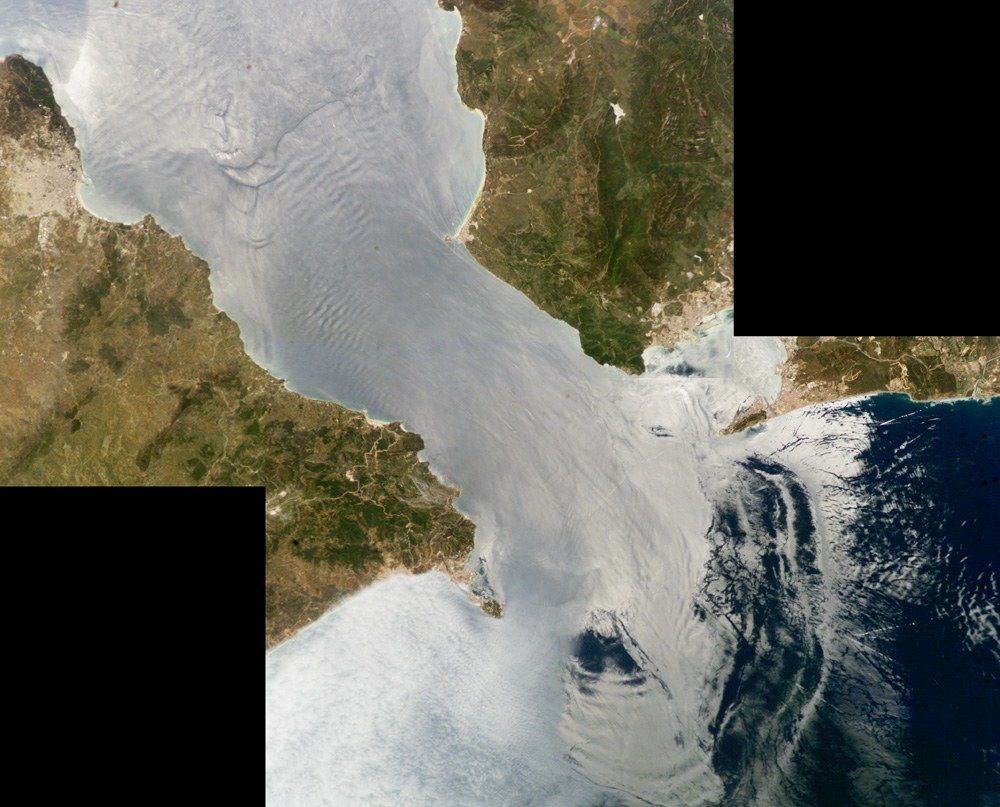
\includegraphics[width=0.72\textwidth]{../figures/al_gibraltar_soliton.jpg}
\caption{孤子是色散与非线性刚好打平的产物：海峡里这列能跨越大洋而不散架的内波，和等离子体中的孤子、非线性波结构遵循同一类平衡。本节先在这张卫星图上建立图像。}
\label{fig:photo-appal2}
\figsource{NASA / 国际空间站宇航员（2004），Public domain（Wikimedia Commons）}
\end{figure}

\section{孤子：色散与非线性平衡}
\label{sec:app-al-soliton}

非线性最容易观察到的结果是\textbf{波形自己变形}：波峰处密度高、折射率高，波峰就追上前面的波谷，
波要倒。色散做相反的事：不同波数的分量跑得快慢不同，波包要摊开。两者恰好抵消时，
波形保持不变——这就是孤子。

离子声波的最小模型是 Korteweg--de Vries 方程，它的单孤子解把振幅与宽度绑在一起：
\begin{equation}
\frac{\delta n}{n_0} = 3(M-1),
\qquad
\Delta = \frac{2\lambda_{De}}{\sqrt{\delta n/n_0}},
\qquad
v_{\mathrm{sol}} = Mc_s .
\label{eq:app-al-kdv}
\end{equation}
取 $M = 1.1$：振幅 $\delta n/n_0 = 0.3$（$30\%$），声速
$c_s = \sqrt{T_e/m_i} = 593524$ m s$^{-1}$ $= 593.524$ km s$^{-1}$，
宽度
\begin{equation}
\Delta = \frac{2\lambda_{De}}{\sqrt{0.3}} = 2.60280\times10^{-4}\ \mathrm{m}
= 260.280\ \mu\mathrm{m},
\label{eq:app-al-solitonwidth}
\end{equation}
即 $\Delta/\lambda_{De} = 3.65148$，孤子速度 $652877$ m s$^{-1}$，
走过自己宽度的时间 $438.533$ ps。\textbf{孤子的宽度是德拜长度的几倍}——这是它能存在的前提：
比德拜长度更细的结构会被Landau 阻尼吃掉，比几十倍德拜长度更宽的结构则来不及平衡非线性。

\begin{table}[htbp]
\centering
\small
\begin{tabular}{p{3.6cm}p{3.4cm}p{4.4cm}}
\toprule
量 & 数值 & 说明 \\
\midrule
马赫数 $M$ & $1.1$ & 超音速才成孤子 \\
相对振幅 $\delta n/n_0$ & $0.3$（$30\%$） & $3(M-1)$ \\
声速 $c_s$ & $593524$ m s$^{-1}$ & $\sqrt{T_e/m_i}$ \\
孤子宽度 $\Delta$ & $260.280$ $\mu$m & $3.65148\,\lambda_{De}$ \\
孤子速度 & $652877$ m s$^{-1}$ & $Mc_s$ \\
特征时间 $\Delta/c_s$ & $438.533$ ps & 走过自身宽度 \\
\bottomrule
\end{tabular}
\caption{离子声孤子：振幅与宽度不是自由参数，由 $M$ 与 $\lambda_{De}$ 定死。}
\label{tab:app-al-soliton}
\end{table}

另一种「非线性挖坑」来自有质动力力：高频场把电子从强场区推出去，留下一个密度凹陷
\begin{equation}
\frac{\delta n}{n} = -\frac{\epsilon_0E^2/2}{4nT_e} = -\frac{W}{4nT_e},
\label{eq:app-al-dent}
\end{equation}
其中 $W = \epsilon_0E^2/2$ 是场能密度。在芯部（$n_e = 10^{20}$ m$^{-3}$、
$T_e = 9.194$ keV），$E = 10^{5}$ V m$^{-1}$ 只挖出 $\delta n/n = 7.51353\times10^{-8}$；
要挖出 $1\%$ 的坑，需要 $E = 3.64820\times10^{7}$ V m$^{-1}$，即功率密度
$1.76643\times10^{12}$ W m$^{-2}$ $= 1.76643\times10^{8}$ W cm$^{-2}$，
折合 $2$ cm 光斑上的 $2.21976$ GW。\textbf{微波做不到，激光可以}——这就是下一节的入口。

\begin{tip}{孤子是平衡，不是「不散」}{tip-app-al-soliton}
孤子常被说成「不散的波包」，这句话省掉了后半句：它不散，是因为\textbf{色散展宽与非线性压缩
每一步都互相抵消}。改温度、改密度、改振幅，平衡就换位置：$T_e$ 降低会把 $\lambda_{De}$
压小，孤子跟着变窄，直到窄到被Landau 阻尼吃掉。孤子不是稳定结构，是\textbf{平衡点}。
\end{tip}

{\footnotesize
\textbf{出处：}离子声孤子的 KdV 解参照 Washimi 与 Taniuti（\emph{Physical Review Letters}
17, 996, 1966）与 Karpman \emph{Nonlinear Waves in Dispersive Media}（1975，第 2--3 章）。
有质动力密度凹陷的量级参照 Max（1973）与 Gibbon \emph{Short Pulse Laser Interactions with
Matter}（2005，第 4 章）。
教科书式的整理参照 Boyd 与 Sanderson \emph{The Physics of Plasmas}
（2003，第 9 章）。
}

\section{参量不稳定性：三波共振与阈值}
\label{sec:app-al-parametric}

「参量」的意思是：一个频率为 $\omega_0$ 的泵浦波，通过\textbf{改变介质的参数}（这里是密度），
把能量交给两个子波。能量与动量都要守恒：
\begin{equation}
\omega_0 = \omega_1 + \omega_2,
\qquad
\mathbf{k}_0 = \mathbf{k}_1 + \mathbf{k}_2 .
\label{eq:app-al-matching}
\end{equation}
两个方程、四个未知数，还要加上两条色散关系才能定解。这是参量过程最容易被讲错的地方：
\textbf{不是任意两个波都能被泵浦起来，必须同时满足频率与波数匹配}。

阈值来自阻尼：子波在长大之前先要克服自己的阻尼，
\begin{equation}
\left(\frac{v_{\mathrm{osc}}}{v_{the}}\right)^{2}
> 4\,\frac{\Gamma_1}{\omega_1}\frac{\Gamma_2}{\omega_2}.
\label{eq:app-al-threshold}
\end{equation}
取 $\Gamma_1/\omega_1 = 10^{-3}$、$\Gamma_2/\omega_2 = 10^{-2}$（电磁波弱阻尼、离子声波强阻尼），
阈值 $v_{\mathrm{osc}}/v_{the} = 6.32456\times10^{-3}$。工作点的
$3.85013\times10^{-3}$ \textbf{低于阈值 $1.64268$ 倍}，对应阈值功率 $P_{th} = 2.69841$ MW：
$1$ MW 的 $140$ GHz 加热在阈值以下，翻到 $2.7$ MW 就会跨过去。这是实验上「功率一高就出现
反常」的定量解释。

同一个判据搬到激光冕区（$T_e = 1$ keV，$v_{the} = 1.32621\times10^{7}$ m s$^{-1}$）：
阈值抖动速度 $83876.6$ m s$^{-1}$，折合强度阈值
$8.74265\times10^{15}$ W m$^{-2}$ $= 8.74265\times10^{11}$ W cm$^{-2}$。
而 ICF 的驱动强度是 $10^{15}$ W cm$^{-2}$ 量级——\textbf{高出三个数量级}，
所以激光等离子体里参量过程不是「可能发生」，而是「一定发生」。

后向受激拉曼散射（SRS）是最重要的一个通道：泵浦光子衰变成一个新光子加一支朗缪尔波。
把匹配条件写成自洽方程
\begin{equation}
k_L = k_0 + k_s,
\qquad
k_s = \frac{\omega_0 - \omega_L(k_L)}{c}\sqrt{1 - \frac{n_e}{n_c}},
\qquad
\omega_L^2 = \omega_{pe}^2 + 3k_L^2v_{the}^2,
\label{eq:app-al-srs}
\end{equation}
在冕区（$k_0 = 1.78531\times10^{7}$ m$^{-1}$、$\omega_0 = 5.38186\times10^{15}$ rad s$^{-1}$）
数值求解得：$k_L = 3.25962\times10^{7}$ m$^{-1}$，即朗缪尔波波长
$\lambda_L = 192.758$ nm，$k_L\lambda_{De} = 0.766278$（冕区 $\lambda_{De} = 23.5082$ nm）
——\textbf{恰好落在Landau 阻尼最强的区间}；散射光波长 $426.177$ nm（斯托克斯位移，
比泵浦的 $350$ nm 长），频率 $707.343$ THz。这三条数放在一起说明一件事：
参量过程把能量交给了一支\textbf{注定要被阻尼掉}的波，所以它是「加热」也是「损失」。

\begin{table}[htbp]
\centering
\small
\begin{tabular}{p{3.4cm}p{3.3cm}p{3.6cm}p{3.4cm}}
\toprule
量 & 微波侧（140 GHz） & 激光冕区（0.35 $\mu$m） & 说明 \\
\midrule
泵浦波数 & $2251.29$ m$^{-1}$ & $1.78531\times10^{7}$ m$^{-1}$ & O 模 \\
阈值判据 & $6.32456\times10^{-3}$ & $8.74265\times10^{11}$ W cm$^{-2}$ & 同一不等式 \\
工作点 & $3.85013\times10^{-3}$ & $10^{15}$ W cm$^{-2}$ & 低于/高于阈值 \\
阈值功率 & $2.69841$ MW & —— & 翻 $1.64268$ 倍即可 \\
子波 1 & 离子声波 & 朗缪尔波 $192.758$ nm & $k_L\lambda_{De} = 0.766278$ \\
子波 2 & 电子波 & 散射光 $426.177$ nm & 斯托克斯位移 \\
\bottomrule
\end{tabular}
\caption{同一套匹配条件与阈值不等式，在两个完全不同的驱动器上给出的答案。}
\label{tab:app-al-parametric}
\end{table}

\begin{tip}{参量过程是「泵浦把能量交给子波」，不是碰撞}{tip-app-al-parametric}
参量不稳定性不需要任何碰撞：它靠的是\textbf{泵浦波自己在介质里造出的密度起伏}。
所以它在无碰撞等离子体里照样发生，而且阈值只由阻尼与功率定——这也解释了为什么
「提高加热功率」有时并不提高加热效率：多出来的功率被参量过程转给了离子声波，
最终进了离子而非电子。
\end{tip}

\textbf{出处：}参量不稳定性与三波耦合的框架参照 Sagdeev 与 Galeev（1969，第 3 章）。
Davidson（1972，第 4--5 章）与 Hasegawa（1975，第 2--3 章）。
激光等离子体中的
受激散射参照 Kruer（1988，第 6--7 章）与 Gibbon（2005，第 5 章）。
阈值与匹配条件的标准写法参照 Boyd 与 Sanderson（2003，第 9 章）。
\begin{figure}[htbp]
\centering
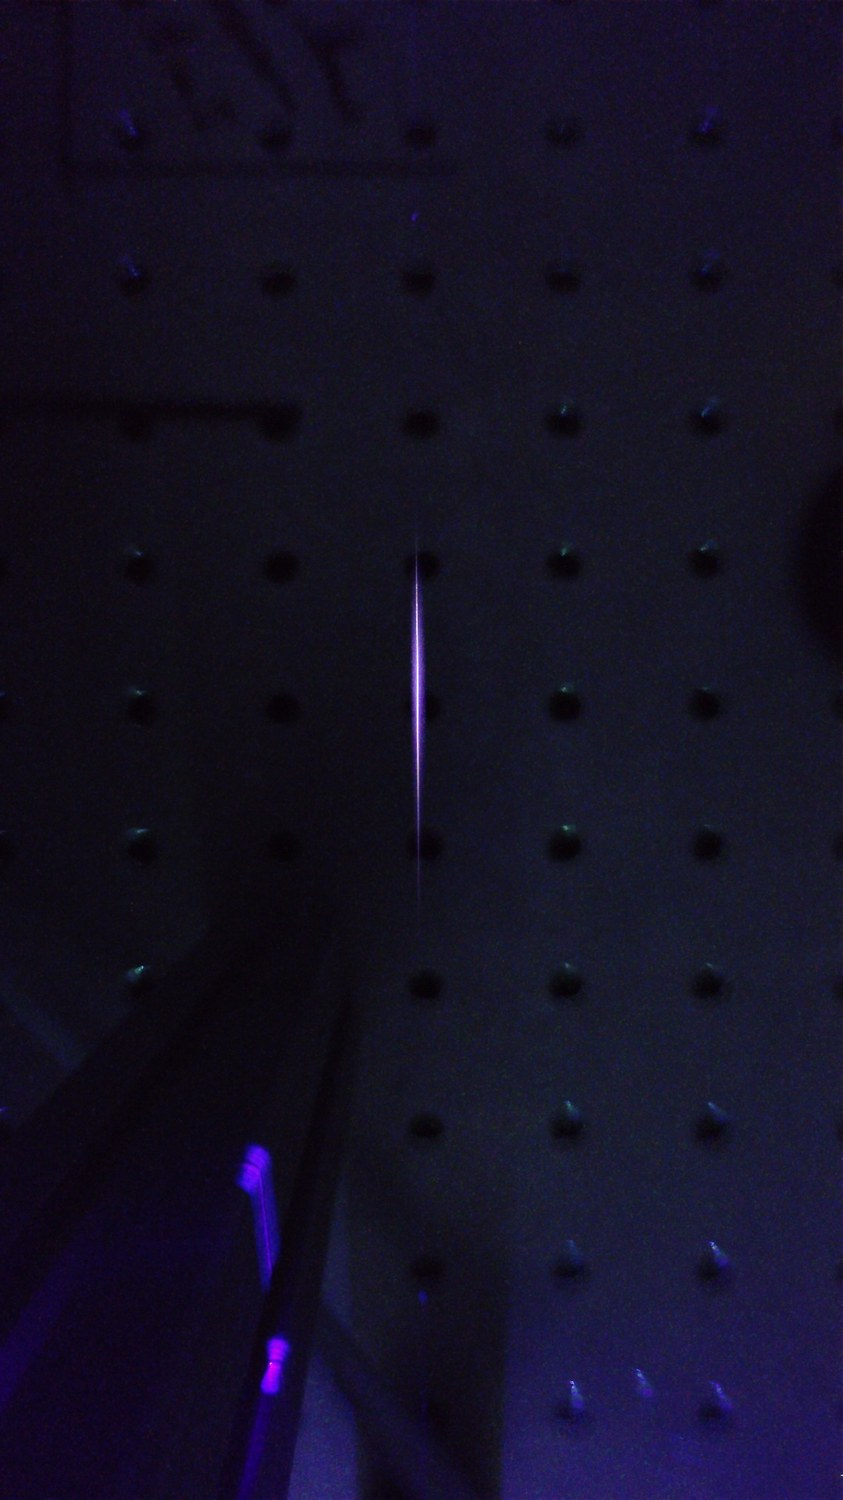
\includegraphics[width=0.52\textwidth]{../figures/al_laser_filament.jpg}
\caption{光强一高，介质的折射率被自己改写，光束就自己收窄成丝——这就是自聚焦。等离子体里的波崩塌吃的是同一套正反馈：本节算的阈值，画面里已经在发生。}
\label{fig:photo-appal3}
\figsource{Jean-Christophe Delagnes，CC BY-SA 4.0（Wikimedia Commons）}
\end{figure}

\section{自聚焦与波崩塌}
\label{sec:app-al-collapse}

上一节的有质动力凹陷一旦足够深，就会出现正反馈：凹陷把波折射进来，进来的波把凹陷挖得更深。
波被自己的密度坑关住了——这就是\textbf{自聚焦}；在三维里继续收缩而不停，就是\textbf{波崩塌}。
判据是一个功率而不是一个场强：
\begin{equation}
P_c = 17.4\,\frac{n_c}{n_e}\ \mathrm{GW},
\label{eq:app-al-pc}
\end{equation}
其中系数 $17.4$ 是量级声明值（相对论与有质动力两种机制的混合，与附录 Y 同口径）。
托卡马克侧：$140$ GHz 的 $n_c/n_e = 2.43127$，于是 $P_c = 4.23041\times10^{10}$ W
$= 42.3041$ GW——\textbf{比 $1$ MW 的加热功率高 $42304.1$ 倍}，自聚焦在磁约束里可以放心忽略。
激光侧：$0.35$ $\mu$m 在 $n_e = 10^{26}$ m$^{-3}$ 的冕区给出 $n_c/n_e = 91.0085$，
$P_c = 1.58355\times10^{12}$ W $= 1.58355$ TW。而 ICF 驱动器峰值功率是 $500$ TW 量级，
是 $P_c$ 的 $315.747$ 倍；即使只算单束（$192$ 束，$2.60417$ TW），也已经是
$P_c$ 的 $1.64451$ 倍。\textbf{这就是为什么激光等离子体里必须谈自聚焦，而磁约束里不必。}

崩塌的空间尺度由德拜长度定：冕区 $\lambda_{De} = 2.35082\times10^{-8}$ m $= 23.5082$ nm，
一个 caviton（约 $10\,\lambda_{De}$）在芯部只有
\begin{equation}
L_{\mathrm{cav}} \sim 10\,\lambda_{De} = 7.12806\times10^{-4}\ \mathrm{m}
= 712.806\ \mu\mathrm{m},
\label{eq:app-al-caviton}
\end{equation}
在冕区则小到 $235.082$ nm。把冕区挖出 $1\%$ 密度坑需要
$E = 1.20317\times10^{10}$ V m$^{-1}$，对应强度 $1.92128\times10^{13}$ W cm$^{-2}$——
比驱动强度低两个数量级，说明\textbf{在 ICF 冕区里密度坑是必然出现的}。

波崩塌到什么时候停止？停在波破裂（wave breaking）：电子在半个周期内被推到与波同速时，
冷等离子体的场上限是
\begin{equation}
E_{WB} = \frac{m_ec\,\omega_{pe}}{e} = 9.61592\times10^{8}\ \mathrm{V\,m^{-1}}
= 961.592\ \mathrm{MV\,m^{-1}}
\label{eq:app-al-ewb}
\end{equation}
（芯部 $n_e = 10^{20}$ m$^{-3}$；$E_{WB}\propto\sqrt{n_e}$，所以附录 Y 里
$10^{24}$ m$^{-3}$ 的固体靶是 $96.1592$ GV m$^{-1}$）。这个上限把非线性从「有序」推向
「耗散」：caviton 崩到 $E_{WB}$ 附近就破裂，把能量交给粒子。

\begin{table}[htbp]
\centering
\small
\begin{tabular}{p{3.4cm}p{3.6cm}p{3.6cm}p{3.2cm}}
\toprule
量 & 托卡马克（140 GHz） & ICF 冕区（0.35 $\mu$m） & 说明 \\
\midrule
$n_c/n_e$ & $2.43127$ & $91.0085$ & 决定 $P_c$ \\
临界功率 $P_c$ & $42.3041$ GW & $1.58355$ TW & $17.4(n_c/n_e)$ GW \\
与驱动功率之比 & $42304.1$（$1$ MW） & $315.747$（$500$ TW） & 差四个数量级 \\
德拜长度 & $71.2806$ $\mu$m & $23.5082$ nm & 决定崩塌尺度 \\
caviton 尺度 & $712.806$ $\mu$m & $235.082$ nm & $\sim10\,\lambda_{De}$ \\
$1\%$ 密度坑所需场 & $3.64820\times10^{7}$ V m$^{-1}$ & $1.20317\times10^{10}$ V m$^{-1}$ & $W/(4nT_e)$ \\
波破裂场 $E_{WB}$ & $961.592$ MV m$^{-1}$ & —— & $\propto\sqrt{n_e}$ \\
\bottomrule
\end{tabular}
\caption{自聚焦与崩塌的两个世界：同一套判据，一个差四个数量级、一个必然发生。}
\label{tab:app-al-collapse}
\end{table}

\begin{tip}{崩塌是「非线性把波自己关起来」}{tip-app-al-collapse}
自聚焦常被误当成「激光太强把物质推开」。顺序正好相反：\textbf{是波先造出密度坑，
密度坑再把波留住}。这也解释了为什么崩塌总发生在功率最高、密度最低的区域：
冕区 $n_c/n_e$ 大，$P_c$ 小，波一进去就跨过门槛。
\end{tip}

{\footnotesize
\textbf{出处：}波崩塌与 caviton 的框架参照 Zakharov（\emph{Soviet Physics JETP} 35, 908, 1972）。
Davidson（1972，第 6 章）与 Hasegawa（1975，第 4 章）。
激光自聚焦与成丝参照
Kruer（1988，第 6 章）与 Gibbon（2005，第 4--5 章）。
波破裂场的标准写法参照
Boyd 与 Sanderson（2003，第 9 章）。
}

\section{粒子俘获：什么时候非线性跑赢阻尼}
\label{sec:app-al-trapping}

前面三节讲的都是\textbf{波与波}的非线性。还有一类同样重要：\textbf{波与粒子}。线性Landau 阻尼说，
速度略慢于相速的粒子吸走波的能量，波按 $e^{-\gamma t}$ 衰减。但这件事有个前提：
粒子在被加速到相速之前，波还来不及衰减。粒子在波的势井里来回振荡的频率是
\begin{equation}
\omega_b = k\sqrt{\frac{eE}{m_e}} ,
\label{eq:app-al-omegab}
\end{equation}
俘获时间 $\tau_{tr} = 2\pi/\omega_b$。与阻尼时间 $1/\gamma$ 比：

\begin{table}[htbp]
\centering
\small
\begin{tabular}{p{2.6cm}p{3.2cm}p{3.2cm}p{4.0cm}}
\toprule
量 & $E = 10^{3}$ V m$^{-1}$ & $E = 10^{4}$ V m$^{-1}$ & 说明 \\
\midrule
俘获频率 $\omega_b$ & $5.58162\times10^{10}$ s$^{-1}$ & $1.76506\times10^{11}$ s$^{-1}$ & $k\sqrt{eE/m_e}$ \\
俘获时间 & $112.569$ ps & $35.5975$ ps & $2\pi/\omega_b$ \\
俘获速度宽度 & $2.65241\times10^{7}$ m s$^{-1}$ & $8.38766\times10^{7}$ m s$^{-1}$ & $2\omega_b/k$ \\
相对热速度 & $0.659596\,v_{the}$ & $2.08582\,v_{the}$ & 势井有多宽 \\
$\omega_b/\gamma$ & $4.38521$ & $13.8672$ & $>1$ 即非线性主导 \\
\bottomrule
\end{tabular}
\caption{粒子俘获与线性阻尼的竞赛（$k\lambda_{De} = 0.3$，$\gamma = 1.27283\times10^{10}$ s$^{-1}$，$1/\gamma = 78.5651$ ps）。}
\label{tab:app-al-trapping}
\end{table}

表 \ref{tab:app-al-trapping} 的结论很硬：只要场强超过
\begin{equation}
E^{*} = \frac{m_e\gamma^2}{k^2e} = 52.002\ \mathrm{V\,m^{-1}},
\label{eq:app-al-ecrit}
\end{equation}
俘获就比阻尼快，线性Landau 阻尼的说法失效。\textbf{$52$ V m$^{-1}$ 是个低得惊人的门槛}——
$1$ MW 的 $140$ GHz 波在芯部给出 $774329$ V m$^{-1}$，是它的上万倍。
把 $k\lambda_{De}$ 从 $0.3$ 提到 $0.5$（波长更短、阻尼更强），门槛升到
$1474.96$ V m$^{-1}$，即 $28.3635$ 倍——\textbf{短波更难被俘获}。

非线性Landau 阻尼的经典结果是 O'Neil 的图景：阻尼不是单调衰减，而是\textbf{先衰减、
再振荡}，振荡频率就是俘获频率，
\begin{equation}
\left\langle E_{\mathrm{wave}}\right\rangle(t)\;\propto\;e^{-\gamma t}\cos(\omega_bt)
\quad\text{（俘获时间尺度上）}.
\label{eq:app-al-oneil}
\end{equation}
所以在强驱动、短波长、低阻尼的实验里，看到阻尼「停住」甚至「回来」并不奇怪：
那是粒子被俘获后开始把能量还回来。

\begin{tip}{俘获把「阻尼」变成「振荡」}{tip-app-al-trapping}
Landau 阻尼之所以显得神秘，是因为它把一个可逆的微观过程（粒子与波交换能量）
伪装成不可逆的宏观衰减。俘获就是把这层伪装撕掉：只要粒子的振荡周期短于衰减时间，
能量就会来回倒——\textbf{阻尼是统计的结果，不是耗散的本质}。
\end{tip}

{\footnotesize
\textbf{出处：}非线性Landau 阻尼与粒子俘获参照 O'Neil（\emph{Physics of Fluids} 8, 2255, 1965）。
Davidson（1972，第 3 章）与 Hasegawa（1975，第 2 章）。
BGK 型平衡态参照
Bernstein、Greene 与 Kruskal（\emph{Physical Review} 108, 546, 1957）。
动理学背景（$\lambda_{De}$、$v_{the}$、Landau 阻尼率）与附录 AE 同口径。
}

\section{相干结构：双电层与相空间空洞}
\label{sec:app-al-structures}

当非线性足够强，等离子体不再由「波」描述，而由\textbf{结构}描述。最常见的两类：

第一类是\textbf{双电层}（double layer）：两层异号空间电荷把电势降集中在一个薄层里。
厚度是德拜长度的一百倍量级，电势降是 $T_e/e$ 量级，于是平均电场
\begin{equation}
E_{\mathrm{dl}} \sim \frac{T_e/e}{100\,\lambda_{De}}
= \frac{9194}{7.12806\times10^{-3}} = 1.28983\times10^{6}\ \mathrm{V\,m^{-1}}
= 12.8983\ \mathrm{kV\,cm^{-1}} .
\label{eq:app-al-dl}
\end{equation}
比同温度下的平均场强高得多，所以在双电层里电子能被一次性加速到 keV 量级——
这是实验室与空间等离子体里「局部加速」的标准机制。

第二类是\textbf{相空间空洞}（phase-space hole）：波把一部分粒子俘获后，分布函数在相空间里
被挖出一个洞，洞本身就是结构，可以比波活得久。洞的宽度就是俘获宽度
\begin{equation}
\Delta v = \frac{2\omega_b}{k} = 8.38766\times10^{7}\ \mathrm{m\,s^{-1}}
= 2.08582\,v_{the}
\qquad (E = 10^{4}\ \mathrm{V\,m^{-1}}),
\label{eq:app-al-hole}
\end{equation}
寿命是 $2\pi/\omega_b = 35.5975$ ps，与 $78.5651$ ps 的线性阻尼时间同量级——
\textbf{结构与被它改造的分布函数寿命相同}。

描述这类结构的两个标准方程值得记住名字：包络近似下电场包络的扎哈罗夫方程
\begin{equation}
\left(i\partial_t + \frac{3}{2}\omega_{pe}\lambda_{De}^2\nabla^2\right)E
= \frac{\omega_{pe}}{2}\frac{\delta n}{n}E ,
\qquad
\left(\partial_t^2 - c_s^2\nabla^2\right)\frac{\delta n}{n}
= \frac{\epsilon_0}{4nT_e}\nabla^2|E|^2 ,
\label{eq:app-al-zakharov}
\end{equation}
以及无碰撞、任意分布函数的 BGK 平衡
\begin{equation}
v\frac{\partial f}{\partial x} + \frac{e}{m_e}\frac{\partial\phi}{\partial x}
\frac{\partial f}{\partial v} = 0
\quad\Longrightarrow\quad
f(x,v) = f\!\left(\tfrac{1}{2}m_ev^2 - e\phi(x)\right) .
\label{eq:app-al-bgk}
\end{equation}
（\ref{eq:app-al-zakharov}）式的第一式说：波的包络被密度凹陷折射；
第二式说：密度凹陷被场的梯度推出来。\textbf{两式合起来就是上一节的自聚焦}。
（\ref{eq:app-al-bgk}）式说：只要分布函数是能量的函数，就是平衡——包括那些
线性理论认为「不该存在」的洞。

\begin{table}[htbp]
\centering
\small
\begin{tabular}{p{3.4cm}p{3.8cm}p{3.6cm}p{3.0cm}}
\toprule
结构 & 尺度 & 特征量 & 寿命 \\
\midrule
双电层 & $100\,\lambda_{De} = 7.12806$ mm & $E = 1.28983$ MV m$^{-1}$ & 稳态（由电流维持） \\
相空间空洞 & $2.08582\,v_{the}$（速度宽度） & $\omega_b = 1.76506\times10^{11}$ s$^{-1}$ & $35.5975$ ps \\
caviton & $\sim10\,\lambda_{De} = 712.806$ $\mu$m & 崩到 $E_{WB}$ 为止 & 几个等离子体周期 \\
孤子 & $3.65148\,\lambda_{De} = 260.280$ $\mu$m & $M = 1.1$ & $438.533$ ps（越过自身） \\
\bottomrule
\end{tabular}
\caption{四种非线性结构的尺度对照：它们的共同点是「比波活得久，比流体元活得短」。}
\label{tab:app-al-structures}
\end{table}

\begin{tip}{相干结构是「自组织」的，不是「外加」的}{tip-app-al-structures}
双电层、空洞、caviton、孤子都不是实验装置的设计产物，而是等离子体在给定能量与
边界条件下\textbf{自己挑出来的形状}。它们出现的意义是：一旦结构形成，
描述语言就从「波的叠加」换成「结构的相互作用」——这也是为什么强非线性区
（冕区、边界、激波下游）很难用线性理论外推。
\end{tip}

{\footnotesize
\textbf{出处：}双电层与相空间空洞的实验与理论综述参照 Sagdeev 与 Galeev（1969，第 4 章）
与 Hasegawa（1975，第 5 章）。
扎哈罗夫方程的原始形式参照 Zakharov（1972）与
Hasegawa 与 Mima（\emph{Physics of Fluids} 21, 87, 1978）。
BGK 模参照
Bernstein、Greene 与 Kruskal（1957）。
无碰撞激波与边界处的结构对照附录 AB 与附录 AD。
\section{估算练习}
\label{sec:app-al-problems}
}

\textbf{练习 1} 把 $2$ MW 的 $140$ GHz 波聚焦到 $12.5664$ cm$^2$（平均功率密度加倍），
求场强与抖动速度，并判断是否达到参量阈值。

\textbf{练习 2} 把强度 $10^{16}$ W cm$^{-2}$、波长 $0.35$ $\mu$m 的激光照到等离子体上，
求归一化振幅 $a_0$ 与有质动力势，并与 $T_e = 9194$ eV 比较。

\textbf{练习 3} 若冕区电子密度升到 $10^{27}$ m$^{-3}$，求 $n_c/n_e$、临界功率 $P_c$
，以及它比 $50$ MW 高多少倍。

\textbf{练习 4} 取 $k\lambda_{De} = 0.5$（短波、阻尼更强），求俘获阈值 $E^{*}$，
以及它比 $k\lambda_{De} = 0.3$ 时高多少倍。

\textbf{练习 5} 在 $0.35$ $\mu$m、$10^{15}$ W cm$^{-2}$ 的冕区里挖出一个 $1\%$ 密度坑，
求所需场强与强度，并说明为什么它低于驱动强度。

\textbf{练习 6} 用后向受激拉曼散射的匹配条件
\begin{equation}
\omega_0 = \omega_s + \omega_L , \qquad
\mathbf{k}_0 = \mathbf{k}_s + \mathbf{k}_L ,
\label{eq:app-al-ex-srs}
\end{equation}
结合电磁波色散 $\omega^2 = \omega_{pe}^2 + k^2c^2$ 与朗缪尔波色散
$\omega_L^2 = \omega_{pe}^2 + 3k_L^2v_{the}^2$，求散射光波长与朗缪尔波波长。

\textbf{解答 1} $S = 2\times7.95775\times10^{8} = 1.59155\times10^{9}$ W m$^{-2}$，
$E = \sqrt{2S/\epsilon_0c} = 1.09507\times10^{6}$ V m$^{-1}$，
$v_{\mathrm{osc}} = eE/(m_e\omega_0) = 218954$ m s$^{-1}$，
于是 $v_{\mathrm{osc}}/v_{the} = 5.44491\times10^{-3}$。它\textbf{仍然低于}阈值
$6.32456\times10^{-3}$——所以把功率翻倍还不够，阈值功率是 $P_{th} = 2.69841$ MW，
即实际功率的 $2.69841$ 倍。

\textbf{解答 2} $a_0 = 0.0299025$，
$U_p = \frac{e^2E^2}{4m_e\omega^2} = 114.292$ eV，
$U_p/T_e = 0.0124312$（芯部 $T_e = 9194$ eV；若取边界温度 $1$ keV，则为 $0.114292$）。\textbf{有质动力势已经超过电子温度的百分之一}，
在激光等离子体里这是个不小的扰动；但和附录 Y 里 $10^{22}$ W cm$^{-2}$ 的
$a_0 = 68.3486$、$U_p = 24.1907$ MeV 相比，还差 20 万倍。

\textbf{解答 3} $n_c/n_e = 9.10085$，
$P_c = 17.4\times9.10085 = 158.355$ GW，
是 $50$ MW 的 $3167.1$ 倍。
换算一下更直观：即使把冕区密度抬高七个量级，自聚焦门槛仍是加热功率的上千倍，
所以\textbf{磁约束装置里永远不必担心自聚焦}。

\textbf{解答 4} $E^{*} = m_e\gamma^2/(k^2e)$，
在 $k\lambda_{De} = 0.5$ 时 $\gamma = 1.12979\times10^{11}$ s$^{-1}$、
$k = 7014.53$ m$^{-1}$，得 $E^{*} = 1474.96$ V m$^{-1}$，
是 $k\lambda_{De} = 0.3$ 时（$52.002$ V m$^{-1}$）的 $28.3635$ 倍。
\textbf{短波更难俘获}：阻尼越强，需要越大的场才能把粒子锁住。

\textbf{解答 5} $1\%$ 密度坑所需场由
\begin{equation}
\frac{\delta n}{n} \simeq \frac{\epsilon_0E^2}{4nT_e}
\label{eq:app-al-ex-dent}
\end{equation}
反解，得 $E = 1.20317\times10^{10}$ V m$^{-1}$，
对应强度 $1.92128\times10^{13}$ W cm$^{-2}$，
是驱动强度（$10^{15}$ W cm$^{-2}$）的 $0.0192128$——\textbf{低两个数量级}。
也就是说，密度坑不是副产品，而是驱动强度随手就挖出来的必然结果。

\textbf{解答 6} 后向散射（$k_s \approx -k_0$ 方向取模）给出
$\omega_L \simeq 2\omega_0 - \omega_{pe}^2/(2\omega_0)$ 量级，
数值解得朗缪尔波 $k_L = 3.25962\times10^{7}$ m$^{-1}$（波长 $192.758$ nm，
$k_L\lambda_{De} = 0.766278$——\textbf{短波、强阻尼区}），
散射光 $k_s = 1.47431\times10^{7}$ m$^{-1}$，波长 $426.177$ nm，
频率 $707.343$ THz。\textbf{散射光在可见光偏蓝一侧，朗缪尔波在紫外}：
这两个波长是可测量的判据。

\section{来源、分级与版权说明}
\label{sec:app-al-source}

\begingroup\small
\textbf{数值分级。}本节把本附录用到的全部数字分三级：

\begin{table}[htbp]
\centering
\small
\begin{tabular}{p{2.2cm}p{4.4cm}p{7.0cm}}
\toprule
级别 & 内容 & 说明 \\
\midrule
现算级 & 抖动速度、有质动力势、阈值、孤子宽度、$P_c$、$E_{WB}$、$\omega_b$、$E^{*}$、双电层场强 & 全部由 \texttt{tools/\allowbreak{}calc/\allowbreak{}appAL\_calc.py} 用 $n_e = 10^{20}$ m$^{-3}$、$T_e = 9194$ eV、$B = 5.3$ T 与声速 $c_s = 593524$ m s$^{-1}$（与附录 AE 同口径）算出 \\
声明级 & 自聚焦系数 $17.4$、孤子形状因子、双电层厚度 $100\,\lambda_{De}$、冕区 $0.35$ $\mu$m 与 $500$ TW 驱动器参数 & 量级或工程典型值，正文中已逐处标为「声明」或「量级」 \\
文献级 & 孤子解（KdV）、三波耦合方程形式、O'Neil 阻尼振荡图景、BGK 平衡、扎哈罗夫方程 & 只引用方程形式与结论，不作数值比对 \\
\bottomrule
\end{tabular}
\caption{}
\label{tab:app-al-source}
\end{table}

\textbf{版权与借鉴口径。}本附录\textbf{不复制}任何原书的文字、编号体系、插图或数据表；
所有数值均由本书自己的脚本独立复算（见表 \ref{tab:app-al-source}），
或明确标注为文献报道值、工程典型值。离线环境下无法逐条核验 DOI，
因此参考文献只给作者、书名或刊名、年份、卷期页；读者需要精确版次时请查原书。
本附录的练习编号与估算流程亦为自拟，\textbf{不复制}任何教材的习题编号体系。

\textbf{借鉴来源。}非线性等离子体物理的框架取自 Sagdeev 与 Galeev
（\emph{Nonlinear Plasma Theory}，1969）。
波与粒子相互作用的处理参照
Davidson（\emph{Methods in Nonlinear Plasma Theory}，1972）与
Hasegawa（\emph{Plasma Instabilities and Nonlinear Effects}，1975）。
孤子与 KdV 的等离子体版本参照 Washimi 与 Taniuti
（\emph{Physical Review Letters} 17, 996, 1966）与 Karpman（1975）。
参量不稳定性与激光等离子体非线性参照 Max（\emph{Physics of Fluids} 16, 1277, 1973）、
Kruer（\emph{The Physics of Laser Plasma Interactions}，1988，第 6--8 章）与
Gibbon（\emph{Short Pulse Laser Interactions with Matter}，2005，第 4--5 章）。
波崩塌与扎哈罗夫方程参照 Zakharov（\emph{Soviet Physics JETP} 35, 908, 1972）与
Hasegawa 与 Mima（\emph{Physics of Fluids} 21, 87, 1978）。
非线性Landau 阻尼参照 O'Neil（\emph{Physics of Fluids} 8, 2255, 1965）与
Bernstein、Greene 与 Kruskal（\emph{Physical Review} 108, 546, 1957），数值与稳定性背景与附录 AC 一致，动理学量与附录 AE 一致，波与不稳定性总览与第 3--4 章、
附录 Y 一致。\textbf{本附录不复制上述文献的任何图表与编号}，只借鉴结论、方程形式与题型。这些文献的推导编号、图表与习题体系一律\textbf{不复制}。

\textbf{与其他附录的分工。}第 3--4 章与附录 Y 讲的是\textbf{线性波与强场}；
本附录补的是「当场强与振幅大到不能线性叠加时，会发生什么」这一层：
孤子（\ref{sec:app-al-soliton}）、参量不稳定性（\ref{sec:app-al-parametric}）、
自聚焦与崩塌（\ref{sec:app-al-collapse}）、粒子俘获（\ref{sec:app-al-trapping}）
与相干结构（\ref{sec:app-al-structures}）。

\begin{tip}{本附录不给什么}{tip-app-al-honest}
本附录\textbf{不给}：三维数值模拟结果、湍流谱的演化、以及非线性饱和的完整理论。
它只做三件事：(1) 用可复算的数字说明非线性何时开始主导。
(2) 给出四类标准非线性过程（孤子、参量、崩塌、俘获）的判据与量级。
(3) 让读者能自己判断「这个问题该不该用线性理论」。
至于饱和之后会发生什么，那要靠模拟，不是靠估算。
\end{tip}
\endgroup
